%% LyX 2.1.3 created this file.  For more info, see http://www.lyx.org/.
%% Do not edit unless you really know what you are doing.
\documentclass[english]{article}
\usepackage[T1]{fontenc}
\usepackage{amssymb}
\usepackage{graphicx}
\usepackage{amsmath}
\usepackage{setspace}
\usepackage{babel}
\begin{document}
\begin{onehalfspace}

\title{Image Processing using Convolutional Neural Networks}
\end{onehalfspace}

\begin{onehalfspace}

\author{Teng Hu, Chengen Xie}
\end{onehalfspace}

\maketitle
\begin{onehalfspace}

\section{Abstract}
\end{onehalfspace}

\begin{onehalfspace}
Defining a specific artistic style has been a controversial topic in both arts and neural science field.  In the paper A Neural Algorithm of Artistic Style. The authors introduce a approach  by using  an artificial system with deep neural network to applied existing art style from a input painting into a new painting.

Our approach is to learn and implement the idea behind the paper and replicates the output. The algorithm captures the style information within different layers of the network, then construct the image that matches the style representation of the given input image. Initially we are planning to use Python to implement the algorithms and utilizing Caffe package to implement the convolution learning network. 

In addition, we tweak the model by implement new layers of learning network, analyze the correspondence between different loss functions and texture representation. 
\end{onehalfspace}


\begin{onehalfspace}

\section{Model Summary}
\end{onehalfspace}

\begin{onehalfspace}
Convolutional neural network is designed to take advantage of the 2D structure of images. CNN consists of a number of convolutional layers and follow by one or more fully connected layers as in standard multilayer neural network. One major benefit is CNN is easier to train and have fewer parameters than fully connected networks with the same number of hidden units.	

The model in the paper is using VGG Network. The model use a publicly available package call caffe-network. p is the original image, and x is the generated image, l is the layer. In each layer in CNN, x is encoded by the filter. The squared-error can be written as following:


It can be derived as:



The input x will change until it converge in the output in a certain layer of the CNN as p. The model also computes the correlation between different filter response above CNN in each layer. As represented by:



To generate texture, the model uses gradient descent from white noise.
In order to mix the image with art style, the model will minimize the distance of a white noise image to match the art style. The total loss of the layer and the total loss is 





To generate the image using the texture the model minimizes the loss function of distance of white noise of the picture and the style from different CNN layers.
\begin{onehalfspace}
\section{Image Process Result}
\end{onehalfspace}

\begin{onehalfspace}
In our project we studied and implemented the model in A Neural Algorithm of Artistic Style, using Torch 7 and VGG-network model in caffe.

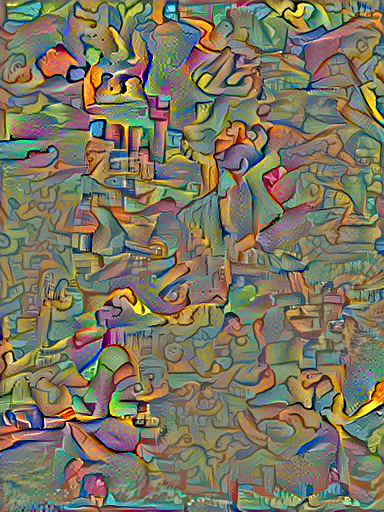
\includegraphics{iter_100.png}
\end{onehalfspace}



\end{onehalfspace}
\begin{onehalfspace}
\section{Conclusion}
\end{onehalfspace}

\begin{onehalfspace}
In our project we studied and implemented the model in A Neural Algorithm of Artistic Style, using Torch 7 and VGG-network model in caffe.

It is well-known that Convolutional Neural Networks are very powerful in Image Processing and already have many interesting applications. The reasons lie in the structure of CNN. Convolutional Neural Networks consist of layers of computational units that process information through feedforward propagation. Each layer of units is a collection of image filters and extracts a different feature of the image. In this paper, the major finding is that the representations of content and style in CNN�
can be separable in layers to some extent, thus we can extract the style of the picture and use it to produce new one combined with other content. In brief, the content of the image we are looking at is referred to positions and arrangement of objects which are stored in high level layers when CNN is trained for object recognition, for the same reason, we can recognize these output images originates from one same image, because our brain recognizes the object unconsciously. On the other hand, the algorithm uses a feature space to store texture information. The feature space consists of correlations between the different filter responses in each layer of network. We extract the style of image by including feature correlations of multiple layers.
\end{onehalfspace}
\end{document}
